\documentclass[conference]{IEEEtran}
\usepackage{ifpdf}
% Heiko Oberdiek's ifpdf.sty is very useful if you need conditional
% compilation based on whether the output is pdf or dvi.
% usage:
% \ifpdf
%   % pdf code
% \else
%   % dvi code
% \fi
% *** CITATION PACKAGES ***
%
\usepackage{cite}
\ifCLASSINFOpdf
  \usepackage[pdftex]{graphicx}
  % declare the path(s) where your graphic files are
  % \graphicspath{{../pdf/}{../jpeg/}}
  % and their extensions so you won't have to specify these with
  % every instance of \includegraphics
  % \DeclareGraphicsExtensions{.pdf,.jpeg,.png}
\else
  % or other class option (dvipsone, dvipdf, if not using dvips). graphicx
  % will default to the driver specified in the system graphics.cfg if no
  % driver is specified.
  \usepackage[dvips]{graphicx}
  % declare the path(s) where your graphic files are
  % \graphicspath{{../eps/}}
  % and their extensions so you won't have to specify these with
  % every instance of \includegraphics
  % \DeclareGraphicsExtensions{.eps}
\fi
\usepackage{amsthm}
\usepackage[ruled,vlined]{algorithm2e}

\usepackage[cmex10]{amsmath}
\usepackage{array}
\usepackage{mdwmath}
\usepackage{mdwtab}
\usepackage{eqparbox}
\usepackage[tight,footnotesize]{subfigure}
\usepackage[caption=false,font=footnotesize]{subfig}
\usepackage{fixltx2e}
\usepackage{stfloats}
% stfloats.sty was written by Sigitas Tolusis. This package gives LaTeX2e
% the ability to do double column floats at the bottom of the page as well
% as the top. (e.g., "\begin{figure*}[!b]" is not normally possible in
% LaTeX2e). It also provides a command:
%\fnbelowfloat
% to enable the placement of footnotes below bottom floats (the standard
% LaTeX2e kernel puts them above bottom floats). This is an invasive package
% which rewrites many portions of the LaTeX2e float routines. It may not work
% with other packages that modify the LaTeX2e float routines. The latest
% version and documentation can be obtained at:
% http://www.ctan.org/tex-archive/macros/latex/contrib/sttools/
% Documentation is contained in the stfloats.sty comments as well as in the
% presfull.pdf file. Do not use the stfloats baselinefloat ability as IEEE
% does not allow \baselineskip to stretch. Authors submitting work to the
% IEEE should note that IEEE rarely uses double column equations and
% that authors should try to avoid such use. Do not be tempted to use the
% cuted.sty or midfloat.sty packages (also by Sigitas Tolusis) as IEEE does
% not format its papers in such ways.
\usepackage{url}
\hyphenation{op-tical net-works semi-conduc-tor}

\begin{document}
%
% paper title
% can use linebreaks \\ within to get better formatting as desired
\title{Bottlenecks in search for Maximal Unique Matches in Suffix Tree}


% author names and affiliations
% use a multiple column layout for up to three different
% affiliations
\author{\IEEEauthorblockN{Julio C\'esar Garc\'ia Vizca\'ino}
\IEEEauthorblockA{Computer Architecture \& Operating Systems Department\\
Universitat Aut\`onoma de Barcelona\\
Bellaterra (Barcelona), Spain\\
Email: jcgarcia@caos.uab.cat}}
%\and
%\IEEEauthorblockN{}
%\IEEEauthorblockA{Twentieth Century Fox\\
%Springfield, USA\\
%Email: homer@thesimpsons.com}
%\and
%\IEEEauthorblockN{James Kirk\\ and Montgomery Scott}
%\IEEEauthorblockA{Starfleet Academy\\
%San Francisco, California 96678-2391\\
%Telephone: (800) 555--1212\\
%Fax: (888) 555--1212}}

% conference papers do not typically use \thanks and this command
% is locked out in conference mode. If really needed, such as for
% the acknowledgment of grants, issue a \IEEEoverridecommandlockouts
% after \documentclass

% for over three affiliations, or if they all won't fit within the width
% of the page, use this alternative format:
% 
%\author{\IEEEauthorblockN{Michael Shell\IEEEauthorrefmark{1},
%Homer Simpson\IEEEauthorrefmark{2},
%James Kirk\IEEEauthorrefmark{3}, 
%Montgomery Scott\IEEEauthorrefmark{3} and
%Eldon Tyrell\IEEEauthorrefmark{4}}
%\IEEEauthorblockA{\IEEEauthorrefmark{1}School of Electrical and Computer Engineering\\
%Georgia Institute of Technology,
%Atlanta, Georgia 30332--0250\\ Email: see http://www.michaelshell.org/contact.html}
%\IEEEauthorblockA{\IEEEauthorrefmark{2}Twentieth Century Fox, Springfield, USA\\
%Email: homer@thesimpsons.com}
%\IEEEauthorblockA{\IEEEauthorrefmark{3}Starfleet Academy, San Francisco, California 96678-2391\\
%Telephone: (800) 555--1212, Fax: (888) 555--1212}
%\IEEEauthorblockA{\IEEEauthorrefmark{4}Tyrell Inc., 123 Replicant Street, Los Angeles, California 90210--4321}}




% use for special paper notices
%\IEEEspecialpapernotice{(Invited Paper)}




% make the title area
\maketitle


\begin{abstract}
  A suffix tree is a data structure very known to solve many classic string matching problems. One problem that can be solved with a suffix tree is the MUM-problem. Assume we are given an alphabet $\Sigma^*$, two sequences R, Q $\in \Sigma^*$, and a number L $>$ 0. The maximal unique matches problem (MUM-problem) is to find all sequences u $\in \Sigma^*$ with: $|u|\geq L$, u occurs exactly once in R and once in Q, and for any character a $\in \Sigma^*$ neither ua nor au occurs both in R and Q. However, the search for MUMs in a suffix tree presents challenges due to irregular and unpredictable data accesses in the suffix tree traversal. This paper analyzes these bottlenecks in the MUM-problem.
\end{abstract}
\IEEEpeerreviewmaketitle



\section{Introduction}
Let's assume the Reference sequence $R[0,\ldots, n-1]$ of size $|R|=n$ over an alphabet $\Sigma={ \$, A, C, G, T}$ which has a sentinel character $R[n-1] = \$$ that occurs nowhere else in the Reference genome and is lexicographically less than all the characters that occur in the alphabet. The suffixes of the Reference genome are zero indexed by their position in the original Reference by a full-text index data structure like a suffix tree. 
\newtheorem{mydef}{Definition}
\begin{mydef}
A suffix tree, $ST$, for an n-character string $R$ is a rooted directed tree with exactly $n$ leaves numbered 0 to n. Each internal node, other than the root, has at least two children and each edge is labeled with a nonempty substring of $R$. No two edges out of a node can have edge-labels beginning with the same character. For any leaf $i$, the concatenation of the edge-labels on the path from the root to leaf $i$ exactly spells out the suffix of $R$ that starts at position $i$. That is, it spells out $R[i\ldots n]$. \cite{Gusfield1997}.
\end{mydef}
A search for a MUM between a Reference, $|R|=n$, and a Query, $|Q|=m$,  can be done in a suffix tree in $O(n+m)$ steps. However it is possible to improve the search for MUMs in a suffix tree by using suffix links \cite{Chang1991}. This improvement reduce the search for MUMs to $O(m)$ steps.

We also define a suffix link, which is an important trick to achieve linear complexity to search for MUMs in both suffix tree.
\begin{mydef}
A suffix link is a pointer from string $\overline{aw}$ to substring $\overline{w}$.
\end{mydef}

\section{Organization of suffix tree in memory}
We use a suffix tree to search for MUMs. It follows an explanation of how suffix tree is stored in memory and how we traverse the suffix tree.

A suffix tree for string x=abab is shown in Figure \ref{suftree}.  
\begin{figure}[!t]
\centering
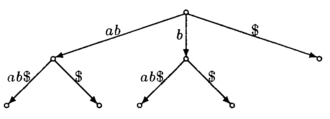
\includegraphics[width=2.5in]{st.png}
\caption{Suffix tree for string x=abab, \cite{Kurtz1999}.}
\label{suftree}
\end{figure}

We use the implementation of a suffix tree suggested in \cite{Kurtz1999} which has two structures: a reference structure which consists of an address pointing a leaf, or to a branching node. The boolean \texttt{toleaf} is \texttt{True} iff \texttt{address} points to a leaf. And a branchinfo structure:
\begin{itemize}
  \item headposition: the head position of the branching node
   \item    depth: the depth of the branching node
  \item suffixlink: the suffix link is always to a branching node
  \item firstchild: the reference to the first child
  \item          branchbrother: the reference to the right brother, if this doesn't exist then it's \texttt{NULL}
\end{itemize}

                             For the suffix tree in Figure \ref{suftree} the tables are shown in Figure \ref{tables}. 
\begin{figure}[!t]
\centering
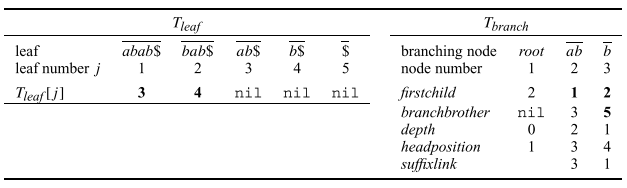
\includegraphics[width=3.5in]{tables.png}
\caption{Tables to store suffix tree for string x=abab, \cite{Kurtz1999}.}
\label{tables}
\end{figure}

The successors of a branching node are therefore found in a list whose elements are linked via the firstchild, branchbrother, and $T_{leaf}$ references. To speed up the access to the successors, each such list is ordered according to the first character of the edge labels. A record component has the following notation: for any component $c$ and any branching node $\overline{w}$, $\overline{w}.c$ denotes the component stored in the branch record $T_{branch}[\overline{w}]$. The head position $j$ of some branching node $\overline{wu}$ tells us that the leaf $\overline{S}_{j}$ occurs in the subtree below node $\overline{wu}$. Hence $wu$ is the prefix of $S_{j}$ of length $\overline{wu}.depth$. As a consequence, the label of the incoming edge to node $\overline{wu}$ can be obtained by dropping the first $\overline{w}.depth$ characters of $wu$, where $\overline{w}$ is the predecessor of $\overline{wu}$.
\newtheorem{myobs}{Observation}

\begin{myobs}
If $\overline{w}\overset{u}{\rightarrow}\overline{wu}$ is an edge in ST and $\overline{wu}$ is a branching node, then we have $u=x_{i}\ldots x_{i+l-1}$ where $i=\overline{wu}.headposition+\overline{w}.depth$ and $l=\overline{wu}.depth-\overline{w}.depth$.
\end{myobs}

Similarly, the label of the incoming edge to a leaf is determined from the leaf number and the depth of the predecessor.

\begin{myobs}
If $\overline{w}\overset{u}{\rightarrow}\overline{wu}$ is an edge in ST and $\overline{wu}=\overline{S}_{j}$ for some $j \in \left[1,n+1\right]$, then $u=x_{i}\ldots x_{n}\$$ where $i=j+\overline{w}.depth$.
\end{myobs}

Every string occurring in a suffix tree $ST$ can uniquely be described in terms of the nodes and edges of $ST$. This is formalized in the notion of \textit{locations}:

\begin{mydef}
Let $ST$ be a suffix tree and $s \in words(ST)$. The \textit{location} of $s$ in $ST$, denoted by $loc_{ST}(s)$ is defined as follows:
\begin{itemize}
\item If $\overline{s}$ is an internal node, then $loc_{ST}(s)=\overline{s}$.
\item If $\overline{s}$ is a leaf in $ST$, then there is a leaf edge $\overline{u}\overset{v}{\rightarrow}\overline{s}$ in $ST$ and $loc_{ST}(s)=(\overline{u},v,\epsilon,\overline{s})$.
\item If there is no node $\overline{s}$ in $ST$, then there is an edge $\overline{u}\overset{vw}{\rightarrow}\overline{uvw}$ in $ST$ such that $s=uv, v\neq \epsilon, w\neq \epsilon$ and $loc_{ST}(s)=(\overline{u},v,w,\overline{uvw})$.
\end{itemize}
\end{mydef}

$locations(ST)=\left\lbrace loc_{ST}(s)|s\in words(ST)\right\rbrace$ is the \textit{set of locations} in $ST$. If a location is a node, we call it \textit{node location}, otherwise \textit{edge location}. Sometimes we identify a node location with the corresponding node.

By convention the \textit{root} is the location of $\epsilon$ in the empty $ST$. The location of a string corresponding to a leaf is not the leaf itself. Instead, it is defined in terms of the edge leading to the leaf. Note that an edge-location $(\overline{u},v,w,\overline{uvw})$ corresponds to a leaf iff $w=\epsilon$. In an edge-location $(\overline{u},v,w,\overline{uvw})$ the string $w$ and the node $\overline{uvw}$ are redundant. Both can uniquely be determined from $\overline{u}$ and $v$ provided the $ST$ is given.

For convenience some additional notions related to locations are introduced.
\begin{mydef}
Given a suffix tree $ST$, suppose $s \in words(ST)$.
\begin{enumerate}
\item $|loc_{ST}(s)|=|s|$ is the $depth$ of the location $loc_{ST}(s)$.
\item Let $v$ be the shortest string s.t. $\overline{sv} \in nodes(ST)$. Then $\overline{sv}$ is denoted by $ceiling(loc_{ST}(s))$.
\item For all $a \in \Sigma$ we define: $occurs(loc_{ST}(s),a)\longleftrightarrow sa$ occurs in $ST$.
\item $rescan(loc_{ST}(s),w)$ denotes $loc_{ST}(sw)$ for all $sw \in words(ST)$.
\end{enumerate}
\end{mydef}

Following a path is the most important operation to search for MUMs. Function $TraverseSuffixTree$ describes this operation.
\begin{mydef}
Let $ST$ be a suffix tree. For each $s \in words(ST)$ and each string $w$ the function $scanprefix: locations(ST)\times\Sigma^{*}\rightarrow locations(ST)\times\Sigma^{*}$ is specified as follows: 
\begin{center}
$TraverseSuffixTree(loc_{ST}(s),w,ST)=(loc_{su},v)$,
\end{center}
where $uv=w$ and $u$ is the longest prefix of $w$ such that $su \in words(ST)$.
\end{mydef}

Moreover, it is very important to have an efficient access from $loc_{ST}(cy)$ to $loc_{ST}(y)$. This access is provided by a function suffixlink, that uses the suffix links of the inner nodes as a "shortcut".
\begin{mydef}
Let $ST$ be a suffix tree. Function suffixlink, $suffixlink:locations(ST)\ \left\lbrace root\right\rbrace\rightarrow locations(ST)$ is defined as:
\begin{center}
$suffixlink(\overline{s})=\overline{z}$
where $\overline{s}\rightarrow\overline{z}$ is the suffix link for $\overline{s}$
\[ suffixlink(\overline{u},av,w,\overline{uavw})= \left\{ 
  \begin{array}{l l}
    loc_{ST}(v) & \quad \text{if $\overline{u}=root$}\\
    rescan(\overline{z},av) & \quad \text{otherwise}
  \end{array} \right.\]
  where $\overline{u}\rightarrow \overline{z}$ is the suffix link for $\overline{u}$
\end{center}
\end{mydef}

\section{Search for MUMs in suffix tree}
Once we have defined the preliminaries in the MUM-problem, we need to answer the question: Where are the MUMs of $R$ and $Q$ of some minimum length $L$? We show the algorithm used to answer this question using a suffix tree, see Algorithm \ref{algST}.
%\linesnumbered
\begin{algorithm}[h]
  \label{algST}
%  \dontprintsemicolon
  \SetKwInOut{Input}{input}
  \SetKwInOut{Output}{output}
  \SetKwData{R}{R}
  \SetKwData{Q}{Q}
  \SetKwData{ST}{ST}
  \SetKwData{Len}{L}
  \SetKwFunction{Length}{length}
  \SetKwData{Leaf}{leaf}
  \SetKwData{MUMs}{MUMs}
  \SetKwData{MUMcands}{MUMcands}
  \SetKwData{loc}{loc}
  \SetKwFunction{buildST}{buildST}
  \SetKwFunction{TraverseSuffixTree}{TraverseSuffixTree}
  \SetKwFunction{suflink}{suffixlink}
  \SetKwFunction{isRootNode}{isRootNode}
  \SetKwFunction{isLeafNode}{isLeafNode}
  \SetKwFunction{saveMUMcand}{saveMUMcand}
  \SetKwFunction{cleanMUMcand}{cleanMUMcand}
  \Input{\R, \Q, \Len}
  \Output{List of \MUMs of \Length$\geq$ \Len, with start position in \R and \Q and \Length}
  \Begin{
  \ST$\leftarrow$ \buildST{\R}\;
  \loc$\leftarrow$ \TraverseSuffixTree{$\Q[0]$,ROOT,\ST}\;
  \For{i=1 to $|Q|$}{
    \If{\isLeafNode{\loc} and \loc.length $\ge$ \Len }{
    \tcc{Leaf saves the position of a suffix in ST.}\;
        \If{$\R[\Leaf-1]\neq \Q[i-1]$}{
            \MUMcands$\leftarrow$ \saveMUMcand{$\R_{\Leaf}$,$i$,\Length}\;
        }
    }
  \eIf{\isRootNode{loc}}{
  \loc$\leftarrow$ \TraverseSuffixTree{$\Q[i+1]$,ROOT,\ST}\;
  }{
  \suflink{\ST,\loc}\;
  \loc$\leftarrow$ \TraverseSuffixTree{$\Q[i+1]$,\loc.node,\ST}\;
  }
  }
  \tcc{Get unique MUMs from list of MUM-candidates.}\;
  \MUMs$\leftarrow$ \cleanMUMcand{\MUMcands}
  }
  \caption{Search for MUMs in a suffix tree.}
\end{algorithm}

In Algorithm \ref{algST} there are two functions related to suffix tree. TraverseSuffixTree performs the traversal of the suffix tree with the current string  and it starts in some given node. suffixlink is a function which gets the suffix link from the current node pointed out by loc.node. If $b$ is an internal node $v$ of suffix tree, then the algorithm can follow its suffix link to a node $s(v)$. If $b$ is not an internal node, then the algorithm can back up to the node $v$ just above $b$. If $v$ is the root, then the search starts in root. But if $v$ is not the root, then the algorithm follows the suffix link from $v$ to $s(v)$.
\section{Suffix tree bottleneck}
Suffix tree is the archetypical index structure used in bioinformatics. For large-scale bioinformatics applications, however, memory consumption really becomes a bottleneck. Moreover, the algorithm to search for MUMs involves comparing the search of a character to the character stored at a specific node at every level of the tree, and traversing a child node based on the comparison results. Only one node at each level is actually accessed, resulting in ineffective cache line utilization, to the linear storage of the tree. Since the result of the comparison is required before loading the appropiate child node, cache line prefetches cannot be issued beforehand. Moreover, meanwhile the Algorithm \ref{algST} shows a $O(m)$ complexity by using suffix links, this feature has the disadvantage of a quite random access to the next node used to traverse the suffix tree. As a consequence a search for MUM typically involves a long-latency TLB/cache miss followed by small number of arithmetic operations at each level of the tree, leading to ineffective utilization of the processor resources.
The best scenario (short-latency and no TLB/cache miss) in a search for MUM is a layout of a whole branch in a cache line size. The worst scenario (long-latency and TLB/cahce miss) is a layout of only one branch read in a cache line size. In Figure \ref{suftree} the suffix tree is implemented with two tables as in Figure \ref{tables}. The layout of branch table has a poor temporal and spatial locality. If string "ba" is searched in the suffix tree by using Algorithm \ref{algST}, then branch node number 1 in Figure \ref{tables} is accessed, it follows an access to branch node number 3 and finally leaf number 3. Use of tables leaf and branch in Figure \ref{tables} helps to traverse a suffix tree, but since each branch node is implemented as a linked list this is a serious performance issue. The linked list have items in disjoint areas of memory. To traverse the list the cache lines cannot be utilized effectively. One could say that the linked list is cache line hostile, or that the linked list maximizes cache line misses. The disjoint memory will make traversing of the linked list slow because RAM fetching will be used extensively.
\subsection{Memory reference locality}
This layout in Figure \ref{tables} of a suffix tree and the random search of strings do not help to a better use of processor resources. The use of suffix links reduces the time complexity of a search for a MUM in a suffix tree but it is not very cache-friendly.

As a proof a poor memory reference locality of this data structure, two experiments were carried out. The features of the computer used are: 2 Processor Intel(R) Xeon(R) E5645 @ 2.4GHz of 6 cores each one, 32KB L1 cache, 256KB L2 and 12MB L3 shared cache per socket. RAM: 96 GB. GCC 4.7.0 with OpenMP support + Linux.

The genomes used were a reference genome of 312Kbp\footnote{Measure unit in DNA genomes.} and 169Mbp, a query genome of 2.91Gbp and a minimum length of MUM of 20bp.

By using the memory heriarchy, we may overlap the latency of a random traversal in a suffix tree. The first experiment is with a small suffix tree (reference of 312Kbp), which is kept in the L3 cache (6MB of memory consumption for suffix tree), the query genome of 2.91Gbp is kept in main memory. The total time to search for MUMs was 149.58 seconds. The second experiment is with a bigger sufffix tree (reference of 169Mbp), which is kept in main memory (3380GB of memory consumption for suffix tree), the query genome of 2.91Gbp is kept in main memory. The total time to search for MUMs was 268.58 seconds. Furthermore, the functions in Algorithm \ref{algST} were profiled to get how many times are accessed in order to have an idea of the bottlenecks while traversing a suffix tree with suffix links. In experiment 1, 6.18\% of times the traversal started in the root of suffix tree. 60.38\% of times suffix links were used. By using suffix links 59.99\% of times the function rescan was used. These measures show how heavy and intensive is the used of suffix links and how it may degrade the performance. In experiment 2, 4.12\% of times the traversal started in the root of suffix tree. 66.47\% of times suffix links were used. In suffix links 69.23\% of times the function rescan was used.
 
%The branch table has the following items, for each branching node $\overline{w}$:
%\begin{itemize}
%\item firstchild refers to the first child of $\overline{w}$.
%\item branchbrother refers to the right brother of $\overline{w}$. If there is no such brother, then branchbrother is a nil reference.
%\item depth is the depth of $\overline{w}$.
%\item headposition is the head position of $\overline{w}$.
%\item suffixlink refers to the branching node $\overline{v}$, if $w$ is of the form $av$ for some $a \in \Sigma$ and some $v \in \Sigma^{*}$.
%\end{itemize}

% An example of a floating figure using the graphicx package.
% Note that \label must occur AFTER (or within) \caption.
% For figures, \caption should occur after the \includegraphics.
% Note that IEEEtran v1.7 and later has special internal code that
% is designed to preserve the operation of \label within \caption
% even when the captionsoff option is in effect. However, because
% of issues like this, it may be the safest practice to put all your
% \label just after \caption rather than within \caption{}.
%
% Reminder: the "draftcls" or "draftclsnofoot", not "draft", class
% option should be used if it is desired that the figures are to be
% displayed while in draft mode.
%


% Note that IEEE typically puts floats only at the top, even when this
% results in a large percentage of a column being occupied by floats.


% An example of a double column floating figure using two subfigures.
% (The subfig.sty package must be loaded for this to work.)
% The subfigure \label commands are set within each subfloat command, the
% \label for the overall figure must come after \caption.
% \hfil must be used as a separator to get equal spacing.
% The subfigure.sty package works much the same way, except \subfigure is
% used instead of \subfloat.
%
%\begin{figure*}[!t]
%\centerline{\subfloat[Case I]\includegraphics[width=2.5in]{subfigcase1}%
%\label{fig_first_case}}
%\hfil
%\subfloat[Case II]{\includegraphics[width=2.5in]{subfigcase2}%
%\label{fig_second_case}}}
%\caption{Simulation results}
%\label{fig_sim}
%\end{figure*}
%
% Note that often IEEE papers with subfigures do not employ subfigure
% captions (using the optional argument to \subfloat), but instead will
% reference/describe all of them (a), (b), etc., within the main caption.


% An example of a floating table. Note that, for IEEE style tables, the 
% \caption command should come BEFORE the table. Table text will default to
% \footnotesize as IEEE normally uses this smaller font for tables.
% The \label must come after \caption as always.
%
%\begin{table}[!t]
%% increase table row spacing, adjust to taste
%\renewcommand{\arraystretch}{1.3}
% if using array.sty, it might be a good idea to tweak the value of
% \extrarowheight as needed to properly center the text within the cells
%\caption{An Example of a Table}
%\label{table_example}
%\centering
%% Some packages, such as MDW tools, offer better commands for making tables
%% than the plain LaTeX2e tabular which is used here.
%\begin{tabular}{|c||c|}
%\hline
%One & Two\\
%\hline
%Three & Four\\
%\hline
%\end{tabular}
%\end{table}


% Note that IEEE does not put floats in the very first column - or typically
% anywhere on the first page for that matter. Also, in-text middle ("here")
% positioning is not used. Most IEEE journals/conferences use top floats
% exclusively. Note that, LaTeX2e, unlike IEEE journals/conferences, places
% footnotes above bottom floats. This can be corrected via the \fnbelowfloat
% command of the stfloats package.


 
\section{Conclusion}
Traverse of suffix tree and use of suffix links are bottlenecks for a better processor performance. In suffix trees larger than the Last Level of Cache, the performance is dictated by the number of cache lines loaded from the memory, and the hardware features available to hide latency due to potential TLB and Last Level of Cache misses.
\section*{Acknowledgment}
This work was supported by grant from "Ejecuci\'on eficiente de aplicaciones multidisciplinares: nuevos desaf\'ios en la era multi/many core", with reference TIN2011-28689-C02-01.

% trigger a \newpage just before the given reference
% number - used to balance the columns on the last page
% adjust value as needed - may need to be readjusted if
% the document is modified later
%\IEEEtriggeratref{8}
% The "triggered" command can be changed if desired:
%\IEEEtriggercmd{\enlargethispage{-5in}}

\bibliographystyle{IEEEtran}
\bibliography{references}
\end{document}


